
%(BEGIN_QUESTION)
% Copyright 2010, Tony R. Kuphaldt, released under the Creative Commons Attribution License (v 1.0)
% This means you may do almost anything with this work of mine, so long as you give me proper credit

Sketch connecting wires to show how to simulate an {\it RTD} signal to the input of this electronic temperature transmitter using a potentiometer:

$$\includegraphics[width=15.5cm]{i03611x01.eps}$$

Assume the transmitter is properly configured for {\bf 4-wire} RTD input, and that the potentiometer is of sufficient precision and resolution that there is no need to connect it to any other resistors to form a network.

\underbar{file i03611}
%(END_QUESTION)





%(BEGIN_ANSWER)

$$\includegraphics[width=15.5cm]{i03611x02.eps}$$

Any correct solution will include these attributes:

\begin{itemize}
\item{} Potentiometer connected as a rheostat (only wiper and one other terminal used, alternatively with third terminal common to wiper)
\item{} Two wires from transmitter to wiper
\item{} Two wires from transmitter to other rheostat terminal
\end{itemize}

%(END_ANSWER)





%(BEGIN_NOTES)

{\bf This question is intended for exams only and not worksheets!}.

%(END_NOTES)


